\documentclass[12pt, titlepage, letterpaper]{article}
%\documentclass[12pt, letterpaper, titlepage]{article}

\usepackage{amsmath}
\usepackage{booktabs}
\usepackage{amsthm}
\usepackage{graphicx}
\usepackage[margin=1in]{geometry}
\usepackage{hyperref}
\hypersetup{colorlinks = true, linkcolor = blue, citecolor=blue, urlcolor = blue}
\usepackage{natbib}
\usepackage{enumitem}
\usepackage{setspace}


\usepackage[]{lineno}
\linenumbers*[1]
% %% patches to make lineno work better with amsmath
\newcommand*\patchAmsMathEnvironmentForLineno[1]{%
 \expandafter\let\csname old#1\expandafter\endcsname\csname #1\endcsname
 \expandafter\let\csname oldend#1\expandafter\endcsname\csname end#1\endcsname
 \renewenvironment{#1}%
 {\linenomath\csname old#1\endcsname}%
 {\csname oldend#1\endcsname\endlinenomath}}%
\newcommand*\patchBothAmsMathEnvironmentsForLineno[1]{%
 \patchAmsMathEnvironmentForLineno{#1}%
 \patchAmsMathEnvironmentForLineno{#1*}}%

\AtBeginDocument{%
 \patchBothAmsMathEnvironmentsForLineno{equation}%
 \patchBothAmsMathEnvironmentsForLineno{align}%
 \patchBothAmsMathEnvironmentsForLineno{flalign}%
 \patchBothAmsMathEnvironmentsForLineno{alignat}%
 \patchBothAmsMathEnvironmentsForLineno{gather}%
 \patchBothAmsMathEnvironmentsForLineno{multline}%
}

% control floats
\renewcommand\floatpagefraction{.9}
\renewcommand\topfraction{.9}
\renewcommand\bottomfraction{.9}
\renewcommand\textfraction{.1}
\setcounter{totalnumber}{50}
\setcounter{topnumber}{50}
\setcounter{bottomnumber}{50}

\newcommand{\jy}[1]{\textcolor{blue}{JY: #1}}
\newcommand{\eds}[1]{\textcolor{red}{EDS: (#1)}}
\newcommand{\mc}[1]{\textcolor{green}{MC: (#1)}}

% NOTE: To produce blinded version, replace "0" with "1" below.
\newcommand{\blind}{1]}

\begin{document}
%\maketitle

\title{\bf Nonparametric Bootstrap Kolmogorov-Smirnov Goodness-of-Fit Test for
  Marginal Distributions of Stationary Time Series}
\if0\blind
{
  \author{Mathew Chandy, %\\
%   \href{mailto:mathew.chandy@uconn.edu}
%   {\nolinkurl{mathew.chandy@uconn.edu}}\\
  Elizabeth Schifano\\
  Jun Yan, %\\
  Xianyang Zhang\\
} \fi


\maketitle


\begin{abstract}

The Kolmogorov-Smirnov (KS) statistic is widely used to test if a sample is
from a given distribution. This study demonstrates how non-parametric 
block bootstrap can be 
used to approximate the KS statistic in situations where parameters are 
not specified and the data are serially dependent. We demonstrate the 
theoretical justication for this method, then through simulation we verify that
it holds it size under the null distribution and is powerful when the null 
hypothesis is false. Finally, we demonstrate applications of the method to
precipitation data from three airports and Microsoft stock returns.

\bigskip
\noindent{\sc Keywords}:
bias-correction; 
dependent data; 
time series. 
\end{abstract}

\doublespace 


\section{Introduction}
\label{sec:intro}

\jy{Start from the need for KS test for stationary series; review existing works
  and identify the gap; summarize the contribution.}

The Kolmogorov-Smirnov (KS) test is a useful goodness-of-fit statistic. 
Let $X_1, ..., X_n$ be a random sample of size~$n$ from some continuous
distribution and the null hypothesis $H_0$ be that $X_i$'s follow the
hypothesized distribution~$F$.
If we let $F_n(t) = \sum_{i=1}^n I(X_i \le t) / n$ be the empirical cumulative
distribution function of the sample, where $I(\cdot)$ is the indicator
function, the KS test statistic takes the form
\begin{equation}
  \label{eq:ks_standard}
  T_n = \sqrt{n} \sup_x | F_{n}(x) - F(x) |.
\end{equation}
As sample size $n\to \infty$, the distribution of $T_n$ converges to that of the
absolute value of standard Brownian bridge, which is known as the Kolmogorov
distribution \citep{stephens1974edf}. The distribution function can be
accurately evaluated in modern statistical software
\citep{marsaglia2003evaluating}. The KS test can be applied to a variety of
fields. \jy{cite a few  references in various field to show its wide
  applications.}
 It has
been used to analyze the random distribution of cosmic microwave background 
radiation \citep{naess2012application}.


Despite its widespread use, the Kolmogorov-Smirnov (KS) test can be 
misapplied when its foundational assumptions are overlooked. The KS test 
assumes the data are independently and identically distributed (i.i.d.) and 
that the hypothesized distribution is continuous and fully specified without 
the need for parameter estimation. \citet{zeimbekakis2022misuses} examines 
common misapplications of the one-sample KS test, notably the inappropriate
use when the hypothesized distribution contains unspecified parameters.
Another commonly encountered situation is when the data are serially
dependent. \citet{babu2004goodness} addresses this issue through the
application of basic non-parametric bootstrap methods. Alternatively, 
\citet{zeimbekakis2022misuses} proposed a semi-parametric bootstrap
where the serial dependence structure is modeled via a working serial copula.
A particularly complex scenario arises when the distribution has unspecified
parameters, and the data are serially dependent. For this,
\citet{zeimbekakis2022misuses} also recommends a semi-parametric bootstrap
approach, where the parameters of the hypothesized distribution and the serial
dependence both need to be estimated and their uncertainty accounted for.


Developing a fully non-parametric solution for the Kolmogorov-Smirnov (KS) 
tests in the presence of serially dependent data presents a significant 
challenge. The null distribution's characteristics are intricately linked to 
the structure of the serial dependence, which can vary widely in practical 
situations. Employing a parametric bootstrap would necessitate defining a 
specific model for this dependence, despite the primary focus being on 
evaluating the marginal distribution of a stationary series. To date, a bias 
correction method for block bootstrap, akin to the approach \citet{babu2004goodness} 
applied to the basic bootstrap, has not been established. This study seeks 
to bridge this gap by introducing a bias correction technique for the 
non-parametric block bootstrap, tailored for use in scenarios where the 
hypothesized distribution includes unspecified parameters and the data 
exhibit serial dependence. Our approach reduces to that of
\citet{babu2004goodness} when the data are independent.


The remainder of this paper is structured as follows: 
Section~\ref{sec:methods} provides an overview of the block bootstrap 
procedure and introduces the bias correction methodology for the 
non-parametric block bootstrap KS test. Section~\ref{sec:simu} is divided 
into two parts; initially, we evaluate the KS test's ability to maintain 
its size, i.e., its consistency in not rejecting the null hypothesis when 
it is indeed true. Subsequently, we examine the test's power, assessing 
whether it can reject the null hypothesis when it is false. Practical 
applications of our method are presented in Section~\ref{sec:real}, where 
we first apply the approach to assess whether annual maximums of hourly 
precipitation at three U.S. airports conform to the Generalized Extreme 
Value (GEV) distribution in Subsection~\ref{sec:precipitation}. Following 
this, we analyze if Microsoft stock return data adhere to either the Normal 
or the Student's $t$ distribution in Subsection~\ref{sec:microsoft}. The 
paper concludes with Section~\ref{sec:conclusion}, offering final thoughts 
and remarks.


\section{Methods}
\label{sec:methods}


Consider a stationary time series $\{X_t: t = 1, \ldots, n\}$ with length~$n$.
We are interested in testing whether or not $X_t$ follows a distribution in a
parametric family of distribution~$F$ indexed by a parameter
vector~$\theta$. That is, the null hypothesis is
\[
  H_0: X_t \sim F(\cdot \mid \theta), \quad t = 1, \ldots, n,
\]
for some unspecified parameter $\theta$.
The alternative hypothesis $H_A$ is that the marginal distribution of $X_t$ does
not follow~$F$ for any parameter value~$\theta$. This is a challenging situation
both the parameters and the serial dependence structure are unknown.


First, let us consider how the KS statistic is typically computed for a sample
with no dependence structure.
Let $\hat\theta_n$ denote the fitted parameters for the hypothesized 
distribution fitted onto $X_t$, and let 
$F_n$ denote the empirical distribution function based on $X_1,...,X_n$
Let
\begin{equation*}
Y_n(x; \hat\theta) = \sqrt{n}(F_n(x) - F(x; \hat\theta_n)).
\end{equation*}
Then, the
goodness of fit statistic is 
\begin{equation*}
T_n := \sup_x|Y_n(x; \hat\theta)|.
\end{equation*}

We note that
\begin{equation*}
Y_n(x; \hat\theta) = \sqrt{n}(F_n(x) - F(x)) - 
\sqrt{n}(F(x; \hat\theta_n) - F(x)),
\end{equation*}
where $F(x)$ is the true cdf (under the null $F(x) = F(x, \theta_0)$ for some
true parameter $\theta_0$).


Let us first consider the case where $X_i$'s are independent. Denote by
$F^{(b)}_n$ the empirical distribution of the $b$th bootstrap sample and let
$\hat\theta^{(b)}_n$ be the parameter estimate based on the $b$th bootstrap 
sample. 
Using the bootstrap (asymptotic) theory, we can approximate the distribution of
$\sqrt{n}(F_n(x) - F(x))$ and $\sqrt{n}(F(x; \hat\theta_n) - F(x))$
by that of $\sqrt{n}(F^{(b)}_n(x) - F_n(x))$ and
$\sqrt{n}(F(x; \hat\theta^{(b)}_n) - F(x; \hat\theta_n))$, respectively.
Therefore, if we define
\begin{align*}
Y^{(b)}_n(x) &= \sqrt{n}(F^{(b)}_n(x) - F_n(x)) - 
               \sqrt{n}(F(x; \hat\theta^{(b)}_n) - F(x; \hat\theta_n)) \\
             &= \sqrt{n}(F^{(b)}_n(x) - F(x; \hat\theta^{(b)}_n)) - 
               \sqrt{n}(F_n(x) - F(x; \hat\theta_n)),
\end{align*}
then $T^{(b)}_n := \sup_x|Y^{(b)}_n(x)|$ is the bootstrap statistic that is 
expected to approximate the distribution of $T_n$. We note that the term
$\sqrt{n}(F_n(x) - F(x; \hat\theta_n))$ is exactly the bias term considered in 
\citet{babu2004goodness}.


We now consider the case where $X_i$'s are realizations from a time series and
$X^{(b)}_1,...,X^{(b)}_n$ are generated by block bootstrap for 
$b \in \{1, \ldots, B\}$.  
Block-bootstrap can be done with overlapping or moving blocks.
Define 
moving blocks (assuming $l > 1$) as:
\begin{equation*}
Z_j =
    \begin{cases}
        \{X_j, \ldots, X_{j + l - 1}\}, & j = 1, \dots, n - l + 1,\\
        \{X_j, \ldots, X_n, X_1, \ldots, X_{j-n+l-1}\}, & j = n - l
        + 2 ,\dots, n.
    \end{cases}
\end{equation*}
A common 
function for block size that is considered optimal is 
$l = \lceil n^{1/3} \rceil$ \citep{buhlmann1999block},  
which was adopted in this study.


We then use bootstrap to approximate the distribuition of
the KS statistic under $H_0$. In this case, we can 
use the distribution of $\sqrt{n}(F^{(b)}_n(x) - E[F^{(b)}_n(x)])$
as an approximation of the distribution of
$\sqrt{n}(F_n(x) - F(x))$,
and the distribution of 
$\sqrt{n}(F(x; \hat\theta^{(b)}_n) - F(x; E[\hat\theta^{(b)}_n]))$ to
approximate $\sqrt{n}(F(x; \theta_n) - F(x))$'s distribution.


We can compute $E[F^{(b)}_n(x)]$ and
$E[\hat\theta^{(b)}_n]$ numerically (they can also be computed analytically, 
depending on the types of block bootstrap we use). One can compute 
$F^{(b)}_n$ 
and $\hat\theta^{(b)}_n$ based on
the $b$th bootstrap sample. Then
$E[F^{(b)}_n(x)] \approx \frac{1}{B}\sum_{b = 1}^BF^{(b)}_n(x)$, and
$E[\hat\theta^{(b)}_n] \approx \frac{1}{B}\sum_{b = 1}^B\hat\theta^{(b)}_n$.
In this case, we can define
\begin{align*}
  Y^{(b)}_n(x) &= \sqrt{n}(F^{(b)}_n(x) - E[F^{(b)}_n(x)]) - 
             \sqrt{n}(F(x; \hat\theta^{(b)}_n) - F(x; E[\hat\theta^{(b)}_n)]) \\
           &= \sqrt{n}(F^{(b)}_n(x) - F(x; \hat\theta^{(b)}_n)) -
             \sqrt{n}(E[F^{(b)}_n(x)] - F(x; E[\hat\theta^{(b)}_n])),
\end{align*}
and $T^{(b)}_n = \sup_x|Y^{(b)}_n(x)|$. Each $T_n^{(b)}$,
$b =1, \ldots, B$, is considered a draw from a distribution that approximates
the distribution of $T_n$. Therefore, the p-value of the observed statistic
$T_n$ can be assessed by positioning it agains the empirical distribution of
$T_n^{(b)}$, $b = 1, \ldots, B$.


In summary, the procedure of the nonparametric block bootstrap test is 
summarized as follows. Repeat the following steps for $b \in \{1, ..., B\}$.
\begin{enumerate}
\item
  Generate $X^{(b)}_1,...,X^{(b)}_n$ by applying moving block bootstrap 
  on the original sample as
  defined previously.
\item
  Fit $F_\theta$ to $X^{(b)}_1,...,X^{(b)}_n$ and obtain estimate 
	$\hat\theta^{(b)}_n$ of $\theta$.
\item
  Obtain the empirical distribution function $F^{(b)}_n$ of
  $X^{(b)}_1,...,X^{(b)}_n$. 
\item
  Calculate bootstrap KS statistic
  \[
    T^{(b)}_n = \sup_x | \sqrt{n}\left(F^{(b)}_n(x) 
    - F(x; \hat\theta^{(b)}_n)\right) - B_n(x) |.
  \]
  where 
  $B_{n}(x) = \sqrt{n}(E[F^{(b)}_n(x)] - 
  F(x; E[\hat\theta^{(b)}_n]))$ is the known
  bias term.
\end{enumerate}


The p-value of the block bootstrap KS test can be computed
as $p = \#\{T^{(b)}_n > T_n\} / B$ for 
$b \in \{1, \ldots, B\}$.

\section{Simulation Studies}
\label{sec:simu}

If we can show that the test correctly fails to reject $H_0$ under the null
distribution, and correctly rejects $H_0$ for an alternate distribution, we can
state that the method works.


\subsection{Size}
We first must evaluate whether this method works when $H_0$ is true. To
test this, we can
generate a simulated sample $X_t$ with a certain marginal distribution 
$F_\theta$,
and use our method to test if $X_t$ indeed has the marginal distribution $F$ 
with some unknown $\theta$. If the test holds its size, the 
p-value
of the test should be uniformally distributed between 0 and 1. We must try the
method with different marginal distributions to ensure that it is robust.
In order for the method to work, a large sample size may be necessary. 


We generated time series with marginal distributions $N(8, 8)$ and
$\Gamma(8, 1)$, Kendall's
\jy{Need to state how serial dependence were introduced, like you did in the
  first paper: transforming a normal series.}
$\tau \in \{-.75, -.5, -.25, 0, .25, .5, 75\}$, and
sample size $n \in \{100, 200, 400, 800\}$. Kendall's $\tau$ was chosen as a
measure of serial dependence as it does not vary between two different 
distributions.
The autocorrelation $\phi$ of the series was set to
$\{-0.924, -0.707, -0.383, 0, 0.383, 0.707, 0.924\}$. These
are the autocorrelations of the normal series, but after the transformation
to the marginal gamma distribution, the autocorrelations are $\{-0.607, 
diverges, -0.287, 0, 0.339, 0.668, 0.911\}$.
\mc{my explanation needs work}


These distributions
were chosen to compare results on normal and non-normal
error structures. The specific parameters were chosen because the distributions 
are very similar and their
first two moments are the same. The series were generated by marginally 
transforming the
marginal normal AR(1) series $X_t$ by
\begin{equation*}
W_t = F^{-1}[\Phi(X_t)],
\end{equation*}
where $F^{-1}(p)$ is the quantile function for the $\Gamma(8, 1)$.
For the purposes of 
evaluating if the test holds it size, when $X_t \sim N(8, 8)$, we tested that the 
marginal distribution family is normal, and when $X_t \sim \Gamma(8, 1)$, we tested
that the marginal distribution family is gamma. For the block bootstrap step,
we used $B = 1000$ and $l = \lceil n^{1/3} \rceil$.
For each setting for $F$, $\tau$, and $n$, we replicate the method 1000 times 
to get the distribution of the p-values 
for the test when applied to samples from the same data generating process.


Using the \textsl{qqplotr} and \textsl{ggplot2} packages 
\citep{qqplotr, ggplot2},
we constructed Q-Q plots of the distribution of the p-values to see if they are
uniformly distributed. If the distribution of the p-values is uniform, this 
indicates that under the null hypothesis, our method will only reject the $H_0$
at a rate of $\alpha$.
A zoomed in plot for probabilities between 0 and 0.1 is
also provided, as
that is the most common range for significance levels $\alpha$. 
%We can also
%compute the rate of rejection $\#P < \alpha$ for different values of
%$\alpha$, as well as a confidence interval
%for this proportion.

\begin{figure}[tbp]
  \centering
  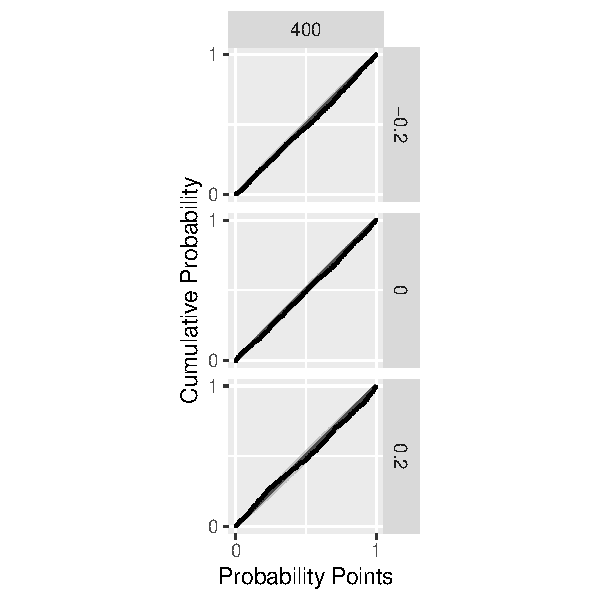
\includegraphics[width = \textwidth]{figures/normal}
  \caption{A Q-Q plot of the p-values testing that a distribution
  generated from a $N(8,8)$ data generating process is normal.}
  \label{fig:normal}
\end{figure}

\begin{figure}[tbp]
  \centering
  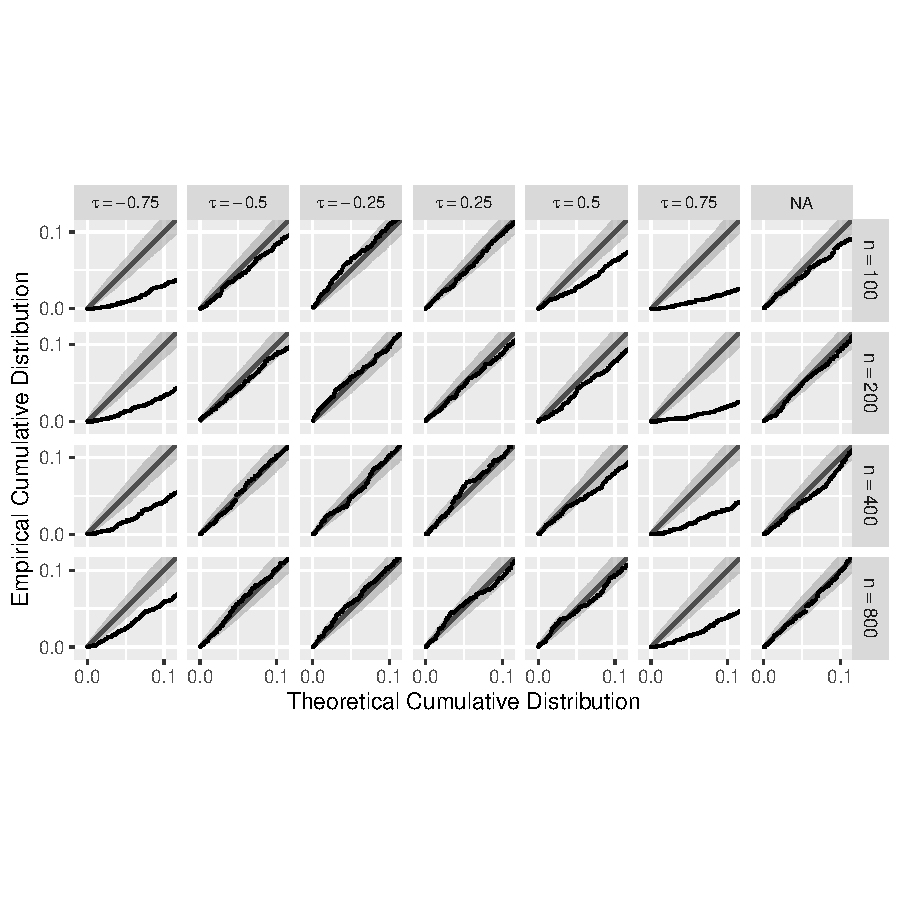
\includegraphics[width = \textwidth]{figures/zoom_normal}
  \caption{A Q-Q plot of the p-values displayed in Figure~\ref{fig:normal} zoomed in to 
  probabilities between 0 and
  0.1}
  \label{fig:zoom_normal}
\end{figure}

\begin{figure}[tbp]
  \centering
  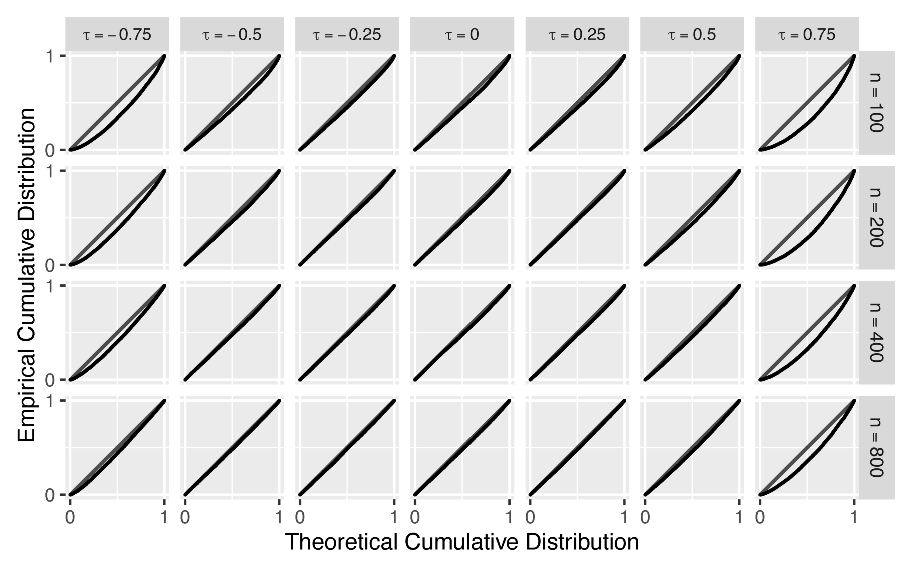
\includegraphics[scale=1]{figures/gamma}
  \caption{A Q-Q plot of the p-values testing that a distribution
  generated from a $\gamma(8,1)$ data generating process is gamma distributed.}
  \label{fig:gamma}
\end{figure}

\begin{figure}[tbp]
  \centering
  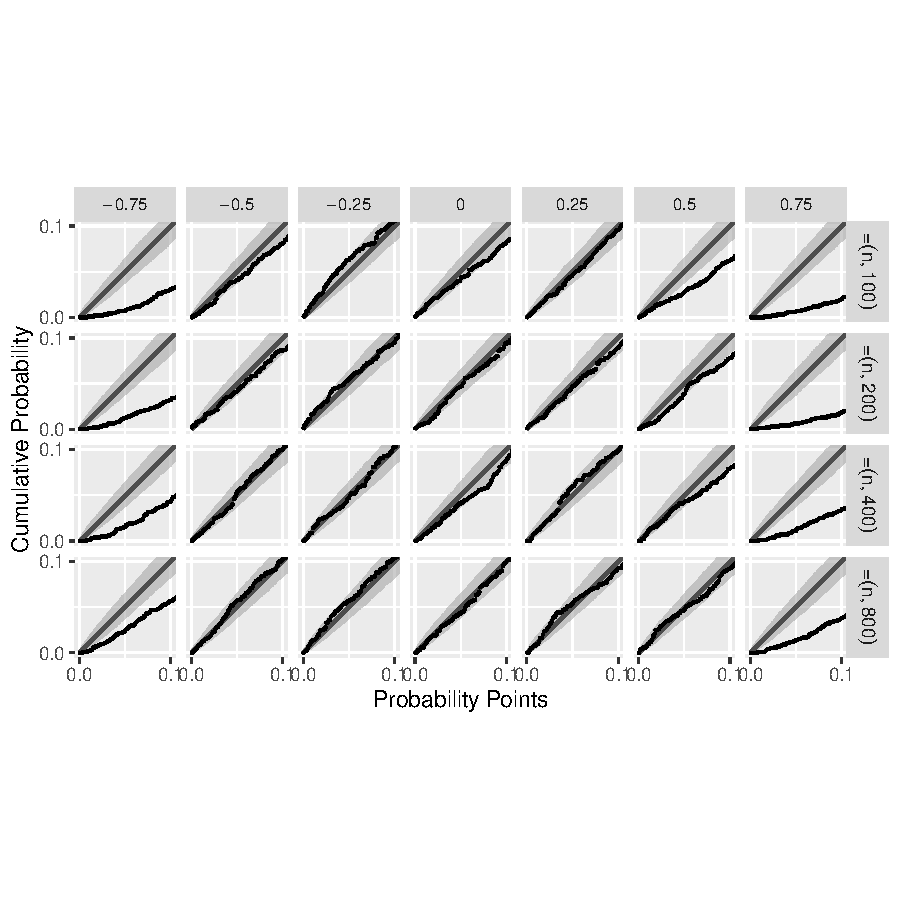
\includegraphics[scale=1]{figures/zoom_gamma}
  \caption{A Q-Q plot of the p-values displayed in Figure~\ref{fig:gamma} zoomed in to 
  probabilities between 0 and
  0.1}
  \label{fig:zoom_gamma}
\end{figure}

From Figures~\ref{fig:normal} and \ref{fig:gamma}, we can observe that 
although the extent to which the p-values appear to be 
completely aligned with the line
in the Q-Q plots is dependent on the sample size and the level of serial 
dependence.
A small sample size like $n = 100$ or $200$ seems adequate when Kendall's
$\tau$ is lower than 0.25. For Kendall's $\tau \geq 0.5$, a sample larger than
$n = 200$ seems necessary for the p-values to be normally distributed. For
Kendall's $\tau \geq 0.75$, a sample larger than $n = 800$ appears to be 
necessary, as the p-values are not aligned with the line in the Q-Q plots, even
in Figures~\ref{fig:zoom_normal} and \ref{fig:zoom_gamma}. This
is not necessarily a cause for concern, as (for normal margins)
a Kendall's $\tau$ corresponds to
a $\phi$ of 0.924, which is very high. Additionally, performance generally seems
better for negative $\tau$ values versus positive $\tau$ values of the same
strength. Results are very similar for normal and gamma margins.


Under $H_0$, the p-values for the non-parametric block bootstrap KS test are
uniformly distributed. This is an indication that our method 
holds its size and that we can expect the probability
of a type 1 error to be the significance level $\alpha$.


\subsection{Power}
We must also evaluate if this method works when $H_0$ is false. We can use
the block bootstrap KS test to test if some $X_t \sim F$ is generated from 
some other 
distribution $G$ with some unknown $\theta$. In this scenario, if the test is 
indeed powerful,
we would ideally want $\beta$ 
(or the probability of failed rejection under $H_A$) 
to be 0, but we
expect it to be generally low. Again, we must try the method with different
marginal distributions to ensure that it is robust.
We would then expect the distribution of p-values to be non-uniform, and the 
rate
of $\#P < \alpha$ to be high, meaning a higher density of low p-values.


Like we did to see if the test holds its size, we generated time series with 
marginal distributions $N(8, 8)$ and 
$\Gamma(8, 1)$, Kendall's $\tau \in \{-.75, -.5, -.25, 0, .25, .5, 
.75\}$, and
sample size $n \in \{100, 200, 400, 800\}$. However, 
to evaluate the test's power, when $X_t \sim N(8, 8)$, we tested that the 
marginal distribution family is gamma. Because the support of $N(8, 8)$ is
$(-\infty, \infty)$, but the support of $\Gamma(8, 1)$ is $(0, \infty)$, we used
the \textsl{truncdist} package \citep{truncdist} to truncate the series at 
values less than or equal to 0.
When $X_t \sim \Gamma(8, 1)$, we tested
that the marginal distribution family is normal. For the block bootstrap step,
we used $B = 1000$ and $l = \lceil n^{1/3} \rceil$.
For each setting for $F$, $\tau$, and $n$, we replicate the method $1000$ times 
to obtain a p-value $p_r$ for each $r \in \{1, \ldots, 1000\}$.


Given some significance level $\alpha$, we can compute a rejection rate 
$q = \#\{p_r < \alpha\} / 1000$ for $r \in \{1, \ldots, 1000\}$.
Additionally, we can construct a 95\% confidence interval for 
this rate. Below are tables containing rejection rates showcasing the 
differences when simulation settings are changed.

\jy{Consider presenting this in a graph. Try explaining the pattern.
  Keep the notations consistent: $n$ and n are different.}


\begin{figure}[tbp]
  \centering
  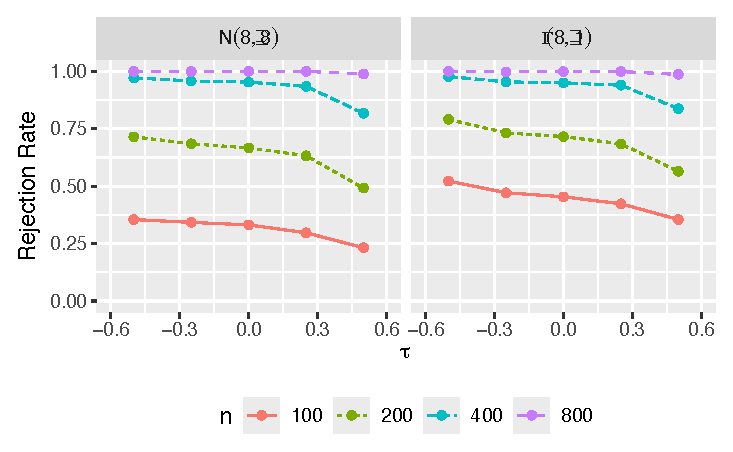
\includegraphics[scale=1]{figures/rr}
  \caption{A plot of the rejection rates as a function of $\tau$ for
 $n \in \{100, 200, 400, 800\}$ and marginal distribution 
 $\in \{N(8,8), \Gamma(8,1)\}$.}
  \label{fig:rr}
\end{figure}


From 
Figure~\ref{fig:rr}, 
the rejection rates appear to get lower as $\tau$ increases in a
positive direction. Using a sample size $n \geq 800$ appears to be sufficient
when $\tau$ is not too high, but for $\tau \geq 0.75$, all sample sizes 
observed appeared to have less than desirable rejection rates. Results
do not appear to be to different when comparing gamma and normal 
margins, indicating that the method is robust to the marginal distribution.


The rejection rates for $n = 800$
are very 
high (almost 1), indicating that under $H_A$, the test is very powerful 
(low probability of failed rejection $\beta$) when a large enough
sample size is used.


\section{Real Data Analysis}
\label{sec:real}

\subsection{Precipitation at Airports}
\label{sec:precipitation}
Annual maximums of hourly precipitation in inches time series data were 
retrieved 
from the Chicago Midway International Airport (MDW), New York LaGuardia 
International 
Airport (LGA),
and Los Angeles International Airport (LAX) stations from the 
National Oceanic and Atmospheric Administration (NOAA). These stations were selected 
from places of importance in the three largest American cities. LGA and
MDW were chosen over John F. Kennedy and O'Hare as more data was available
from these stations. The data for MDW is from
1948 to 2014, the data for LGA is from 1948 to 2013, and the
data for LAX is also from 1948 to 2013. We can apply our method (as well
as the non-parametric bootstrap KS Test \citep{babu2004goodness} and
the parametric bootstrap KS Test) to
the precipitation time series from each of these locations to test if they
follow the
Generalized Extreme Value (GEV) distribution using the \textsl{evd} 
package \citep{evd}. Precipitation maximum series 
typically do follow the GEV distribution, so we expect to fail to reject the
null hypothesis.

\jy{Is the parametric method by Zeimberkakis?}

%% latex table generated in R 4.3.0 by xtable 1.8-4 package
% Sun Feb 25 12:46:58 2024
\begin{table}[ht]
\centering
\caption{P-values for testing that annual maximums of hourly 
            precipitation from the three airports follows the GEV distribution.} 
\label{table:precipitation}
\begin{tabular}{rrrr}
  \hline
 & block & basic & param \\ 
  \hline
MDW & 0.16 & 0.21 & 0.08 \\ 
  LGA & 0.44 & 0.55 & 0.48 \\ 
  LAX & 0.28 & 0.36 & 0.34 \\ 
   \hline
\end{tabular}
\end{table}


%\mc{https://hdsc.nws.noaa.gov/pfds/pfds_map_cont.html?bkmrk=ct}

The p-value is 0.71 for MDW, 0.13 for LGA, and 0.36 for LAX when using our 
method.
When using Babu's non-parametric method which does not account for serial
dependence, the p-value is 0.74 for MDW, 0.19 for LGA, and 0.40 for LAX. 
When using the parametric bootstrap KS test, the p-value is 0.64 for MDW,
0.12 for LGA, and 0.35 for LAX. In this instance, the conclusions are the
same 
(the three series follow the GEV distribution), but because of the difference
in p-values, it is possible for different conclusions to be found in another
study.

\subsection{Temperature in Central Park}
\label{sec:temperature}

Annual temperature maximums recorded in Central Park, New York, NY from
1895 to 2023 were sourced from the NOAA. Again, we are interested in seeing
if our method, which
accounts for serial dependence and does not require parameter specification,
performs differently than the non-parametric bootstrap KS Test 
\citep{babu2004goodness} and the parametric bootstrap KS Test, neither of
which account for serial dependence. We found that when using our method,
the p-value for the test that the series follows the GEV distribution is 0.1420.
When using Babu's method, the p-value is 0.0666, and when using the parametric
method, the p-value is 0.0682. At the common significance level of .05,
the conclusions would be the same regardless of the method used. However, it
is clear that for this series, our method more decisively fails to reject the 
null hypothesis at a significance level of .10.

\jy{Sorry I forgot to send you the data I promised. Remind in the future
  please. }

\subsection{Microsoft Stock Returns}
\label{sec:microsoft}

%\mc{https://www.nasdaq.com/market-activity/stocks/msft/historical}

We expect the marginal distribution of Microsoft stock returns to have a 
slightly
heavier tail than the normal distribution. Using the \textsl{tseries} package 
\citep{tseries}, 
we gathered closing stock prices from January 1st, 1998 to December 31st, 2022.
Then we approximated stock returns by taking the difference in the logarithm 
of the closing prices.
We tested that the stock returns are normally
distributed (which we expect to reject).  After that, we tested that the
marginal distribution of the time series follows the Student's $t$ distribution
with a fixed degrees of freedom.
While we 
could choose to estimate a fitted value of the degrees of freedom parameter $v$
as
part of our method, it is very difficult to do so. Therefore, we attempted to
test 
if it follows
the location-scale $t$ distribution with increasingly smaller specified degrees 
of freedoms. This was achieved with the \textsl{extraDistr} 
package \citep{extraDistr}. We
also observed how the method performs using increasingly smaller durations of
time. ,
we used the last 5 years of data: January 1st, 2018 to December 31st, 2022,
4 years of data: January 1st, 2019 to December 31st, 2022,
3 years of data: January 1st, 2020 to December 31st, 2022,
2 years of data: January 1st, 2021 to December 31st, 2022,
and 1 year of data: January 1st, 2022
to December 31st, 2022. In addition, we compared it to results from 
the Babu non-parametric and 
the parametric bootstrap KS Test.


% latex table generated in R 4.3.0 by xtable 1.8-4 package
% Sun Feb 25 11:43:59 2024
\begin{table}[ht]
\centering
\caption{P-values for 1 year of Microsoft stock return data using different 
  methods
  and different degrees of freedom for Student's t distribution.} 
\label{table:microsoft1}
\begin{tabular}{rlllll}
  \hline
 & duration & df & block & basic & param \\ 
  \hline
1 & 1 & norm & 0.556 & 0.573 & 0.511 \\ 
  2 & 1 & 30 & 0.595 & 0.606 & 0.585 \\ 
  3 & 1 & 20 & 0.609 & 0.624 & 0.627 \\ 
  4 & 1 & 10 & 0.654 & 0.67 & 0.671 \\ 
  5 & 1 & 5 & 0.572 & 0.596 & 0.569 \\ 
  6 & 1 & 4 & 0.394 & 0.417 & 0.42 \\ 
  7 & 1 & 3 & 0.219 & 0.214 & 0.217 \\ 
  8 & 1 & 2 & 0.094 & 0.101 & 0.111 \\ 
  9 & 1 & 1 & 0.001 & 0.002 & 0.004 \\ 
   \hline
\end{tabular}
\end{table}



% latex table generated in R 4.3.0 by xtable 1.8-4 package
% Sun Feb 25 11:43:59 2024
\begin{table}[ht]
\centering
\caption{P-values for 2 years of Microsoft stock return 
                   data using different durations
  and different degrees of freedom for Student's t distribution.} 
\label{table:microsoft2}
\begin{tabular}{rlllll}
  \hline
 & duration & df & block & basic & param \\ 
  \hline
1 & 2 & norm & 0 & 0.002 & 0 \\ 
  2 & 2 & 30 & 0.001 & 0.003 & 0.001 \\ 
  3 & 2 & 20 & 0.001 & 0.005 & 0.002 \\ 
  4 & 2 & 10 & 0.005 & 0.018 & 0.003 \\ 
  5 & 2 & 5 & 0.008 & 0.021 & 0.009 \\ 
  6 & 2 & 4 & 0.01 & 0.021 & 0.015 \\ 
  7 & 2 & 3 & 0.021 & 0.029 & 0.029 \\ 
  8 & 2 & 2 & 0.01 & 0.016 & 0.014 \\ 
  9 & 2 & 1 & 0 & 0 & 0 \\ 
   \hline
\end{tabular}
\end{table}



% latex table generated in R 4.3.0 by xtable 1.8-4 package
% Mon Feb 12 23:32:06 2024
\begin{table}[ht]
\centering
\caption{P-values for 3 years of Microsoft stock return 
                   data using different durations
  and different degrees of freedom for Student's t distribution.} 
\label{table:microsoft3}
\begin{tabular}{rlllll}
  \hline
 & duration & df & block & basic & param \\ 
  \hline
1 & 3 & norm & 0 & 0 & 0 \\ 
  2 & 3 & 30 & 0.001 & 0 & 0 \\ 
  3 & 3 & 20 & 0.001 & 0 & 0 \\ 
  4 & 3 & 10 & 0.001 & 0.001 & 0 \\ 
  5 & 3 & 5 & 0.097 & 0.095 & 0.096 \\ 
  6 & 3 & 4 & 0.273 & 0.274 & 0.283 \\ 
  7 & 3 & 3 & 0.115 & 0.133 & 0.129 \\ 
  8 & 3 & 2 & 0.014 & 0.024 & 0.021 \\ 
  9 & 3 & 1 & 0 & 0 & 0 \\ 
   \hline
\end{tabular}
\end{table}



% latex table generated in R 4.3.0 by xtable 1.8-4 package
% Mon Feb 12 23:32:06 2024
\begin{table}[ht]
\centering
\caption{P-values for 4 years of Microsoft stock return 
                   data using different durations
  and different degrees of freedom for Student's t distribution.} 
\label{table:microsoft4}
\begin{tabular}{rlllll}
  \hline
 & duration & df & block & basic & param \\ 
  \hline
1 & 4 & norm & 0 & 0 & 0 \\ 
  2 & 4 & 30 & 0 & 0 & 0 \\ 
  3 & 4 & 20 & 0 & 0 & 0 \\ 
  4 & 4 & 10 & 0 & 0 & 0 \\ 
  5 & 4 & 5 & 0.004 & 0.001 & 0.002 \\ 
  6 & 4 & 4 & 0.032 & 0.041 & 0.049 \\ 
  7 & 4 & 3 & 0.06 & 0.1 & 0.114 \\ 
  8 & 4 & 2 & 0.006 & 0.006 & 0.009 \\ 
  9 & 4 & 1 & 0 & 0 & 0 \\ 
   \hline
\end{tabular}
\end{table}



% latex table generated in R 4.3.0 by xtable 1.8-4 package
% Mon Feb 12 23:32:06 2024
\begin{table}[ht]
\centering
\caption{P-values for 5 years of Microsoft stock return 
                   data using different durations
  and different degrees of freedom for Student's t distribution.} 
\label{table:microsoft5}
\begin{tabular}{rlllll}
  \hline
 & duration & df & block & basic & param \\ 
  \hline
1 & 5 & norm & 0 & 0 & 0 \\ 
  2 & 5 & 30 & 0 & 0 & 0 \\ 
  3 & 5 & 20 & 0 & 0 & 0 \\ 
  4 & 5 & 10 & 0 & 0 & 0 \\ 
  5 & 5 & 5 & 0.001 & 0 & 0.001 \\ 
  6 & 5 & 4 & 0.008 & 0.002 & 0.008 \\ 
  7 & 5 & 3 & 0.021 & 0.015 & 0.024 \\ 
  8 & 5 & 2 & 0 & 0.002 & 0.002 \\ 
  9 & 5 & 1 & 0 & 0 & 0 \\ 
   \hline
\end{tabular}
\end{table}



\jy{Report the autocorrelation estimate of residual and residual squared in the
  text.}



The p-values of our test when applied to Microsoft stock return data using
different settings are showcased in 
Tables~\ref{table:microsoft1}--\ref{table:microsoft2}. Although the p-values
are indeed different between the three methods, the conclusions at a .05 
significance 
level are mostly the same. This motivated an additional application on SP500
and SP100 data.



\section{Concluding Remarks}
\label{sec:conclusion}

Using simulation, we have shown that given a large enough sample of a time 
series, the block 
bootstrap KS test can appropriately fail to reject the null hypothesis when the
series follows the null distribution. In addition, when the marginal
distribution is not
the one hypothesized, the test is powerful. It requires a larger sample size 
than basic bootstrap to avoid either type I or type II errors. Unsurprisingly,
the method performs better as the temporal dependence gets weaker. Through
simulation studies with Normal and Gamma-distributed data, we have shown that
that the method is robust. We have also 
demonstrated possible applications of this method to precipitation and 
stock return data. This method can be used for any study where the goal is
to see if a time series follows a hypothesized distribution and the parameters
are unknown or unspecified. Future studies could apply the method showcased
in this paper to fields like earthquake prediction and astronomy.


\jy{The number of references seems low. Need to cite more related works.}


\jy{Quality control the bib source}

\bibliographystyle{asa}
\bibliography{citations}


\end{document}
%%% LocalWords: nonparametric semiparametric autocorrelation ARMA
%%% Local Variables:
%%% mode: latex
%%% TeX-master: t
%%% ispell-personal-dictionary: ".aspell.en.pws"
%%% fill-column: 80
%%% eval: (auto-fill-mode 1)
%%% End: